
%%% Local Variables:
%%% mode: latex
%%% TeX-master: "../Tesis"
%%% End:
\chapter{Particle Accelerators}
\label{c:accel} % For referencing the chapter elsewhere, use \ref{} 
\lhead{Chapter~\ref{c:accel}.
  Accelerators} % This is for the header on each page - perhaps a shortened title
Particle accelerators are machines whose name is self explanatory, and were
originally developed for nuclear physics. Although we could argue that a
cathodic tube is an accelerator itself, we count as the first accelerator one
that was designed, after Rutherford challenged the scientific community in 1927
to accelerate charged particles to energies higher than natural
$\alpha$-decays\cite{Steere2005timeline}, which have a typical energy of
\SI{5}{MeV} \rojo{I am currently using the \textbackslash{}SI\{\}\{\}, but
  shouldn't there be a space between units and unit?}, this accelerator was the
\cite{Cockroft619}

\begin{figure}
	\centering
  \begin{minipage}{\textwidth}
  	\centering
   	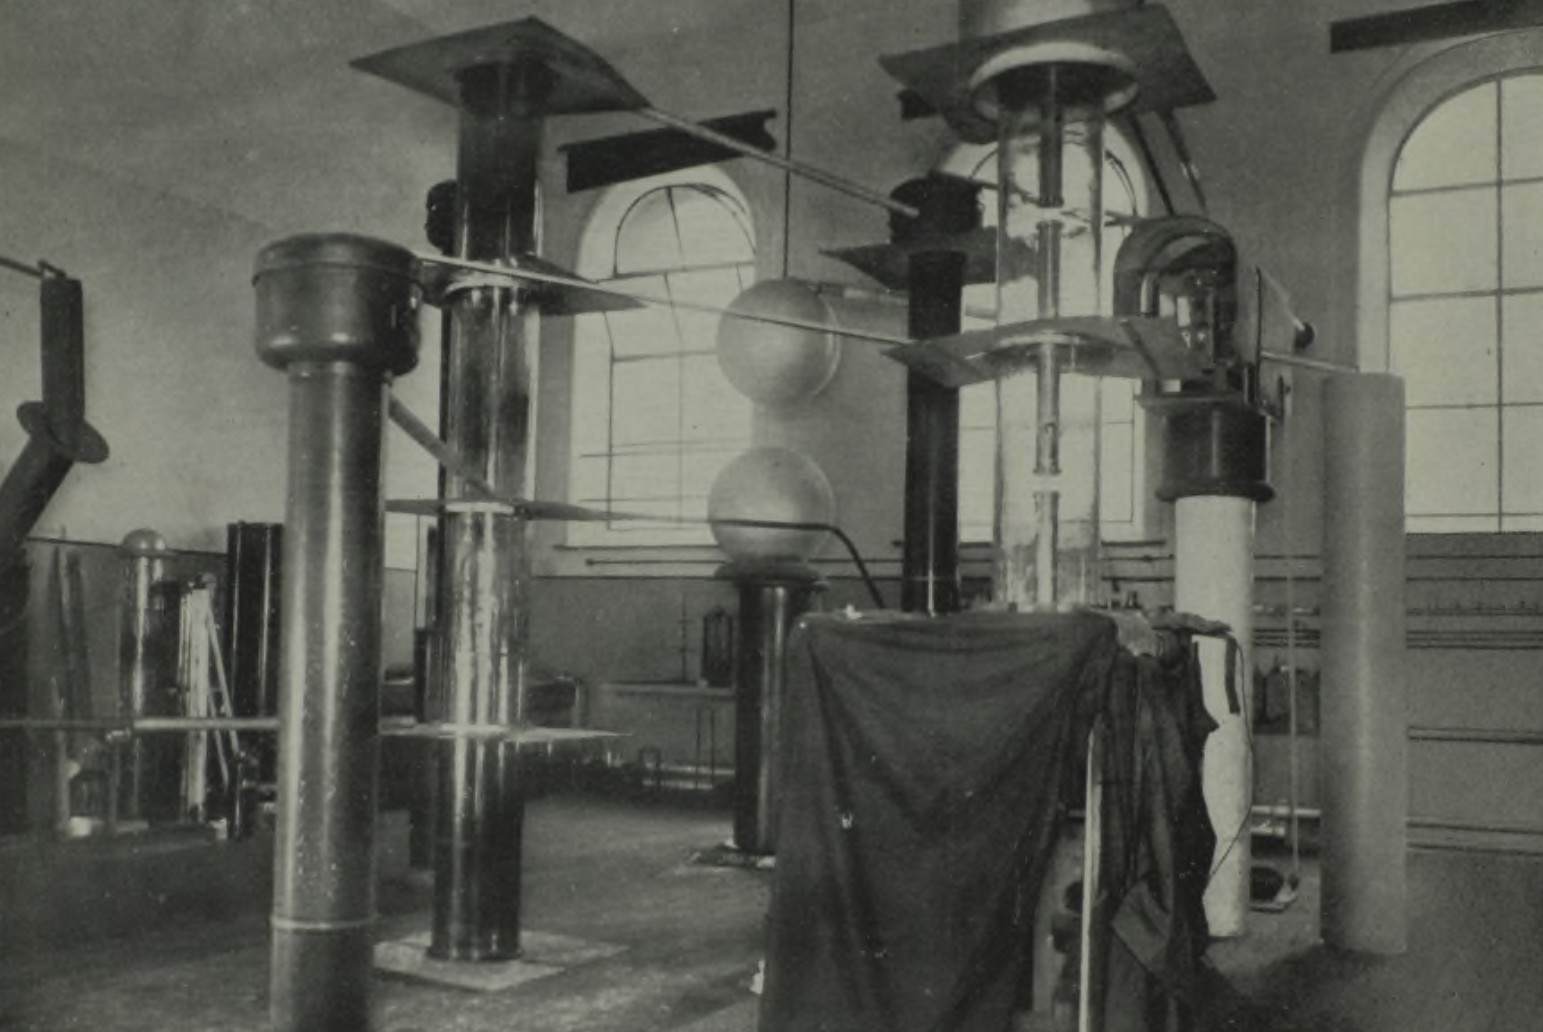
\includegraphics[width=3.5in]{Pictures/cockroft.png}
  		\caption{\label{fig:cock}
   			Cockroft-Walton accelerator original setting.}
   			\footnotesize{Picture taken from \citep{Cockrofft619}}
   \end{minipage}
\end{figure}

\section{Working Principles}

\section{LHC}
\subsection{HL-LHC}
\section{FCC}
\subsection{HE-LHC}
\subsection{FCC-hh}
\subsection{FCC-ee}
\subsection{FCC-he}
